% -*- TeX:de -*-
\NeedsTeXFormat{LaTeX2e}
\documentclass[12pt,a4paper]{article}
\usepackage[german]{babel} % german text
\usepackage[DIV12]{typearea} % size of printable area
\usepackage[T1]{fontenc} % font encoding
%\usepackage[latin1]{inputenc} % most likely on Windows
\usepackage[utf8]{inputenc} % probably on Linux
\usepackage{multicol}

% PLOTTING
\usepackage{pgfplots} 
\usepackage{pgfplotstable}
\usepackage{url}
\usepackage{graphicx} % to include images
\usepackage{tikz}
\usepackage{subfigure} % for creating subfigures
\usepackage{amsmath} % a bunch of symbols
\usepackage{amssymb} % even more symbols
\usepackage{booktabs} % pretty tables
\usepackage{makecell} % multi row table heading

% a floating environment for circuits
\usepackage{float}
\usepackage{caption}

%\newfloat{circuit}{tbph}{circuits}
%\floatname{circuit}{Schaltplan}

% a floating environment for diagrams
%\newfloat{diagram}{tbph}{diagrams}
%\floatname{diagram}{Diagramm}

\selectlanguage{german} % use german

\begin{document}








%%%% TO DO
%
% - - Shorty:
%
% - - Tabelle "Messwerte Linsenbrennweite"
%		bitte bei jedem neuen e eine trennlinie... bin zu deppert ^^

% - - Patrick
%




%%%%%%% DECKBLATT %%%%%%%
\thispagestyle{empty}
			\begin{center}
			\Large{Fakultät für Physik}\\
			\end{center}
\begin{verbatim}


\end{verbatim}
							%Eintrag des Wintersemesters
			\begin{center}
			\textbf{\LARGE WS 2013/14}
			\end{center}
\begin{verbatim}


\end{verbatim}
			\begin{center}
			\textbf{\LARGE{Physikalisches Praktikum\\ für das Bachelorstudium}}
			\end{center}
\begin{verbatim}




\end{verbatim}

			\begin{center}
			\textbf{\LARGE{PROTOKOLL}}
			\end{center}
			
\begin{verbatim}





\end{verbatim}

			\begin{flushleft}
			\textbf{\Large{Experiment (Nr., Titel):}}\\
							%Experiment Nr. und Titel statt den Punkten eintragen
			\LARGE{PW7 Brechung, Dispersion, Refraktometrie}	
			\end{flushleft}

\begin{verbatim}

\end{verbatim}	
							%Eintragen des Abgabedatums, oder des Erstelldatums des Protokolls
			\begin{flushleft}
			\textbf{\Large{Datum:}} \Large{21.11.2013}
			\end{flushleft}
			
\begin{verbatim}
\end{verbatim}
							%Namen der Protokollschreiber
		\begin{flushleft}
			\textbf{\Large{Namen:}} \Large{Patrick Braun, Johannes Kurz}
			\end{flushleft}

\begin{verbatim}


\end{verbatim}
							%Kurstag und Gruppennummer, zb. Fr/5
			\begin{flushleft}
			\textbf{\Large{Kurstag/Gruppe:}} \Large{DO/2}
			\end{flushleft}

\begin{verbatim}



\end{verbatim}
							%Name des Betreuers, das Praktikum betreute.
			\begin{flushleft}
			\LARGE{\textbf{Betreuer:}}	\Large{ Johanna Akbarzadeh }	
			\end{flushleft}

%%%%%%% DECKBLATT ENDE %%%%%%%
\pagebreak
\setlength{\columnsep}{20pt}
\begin{multicols}{2}


%\begin{figure}[H]
%	\centering
%	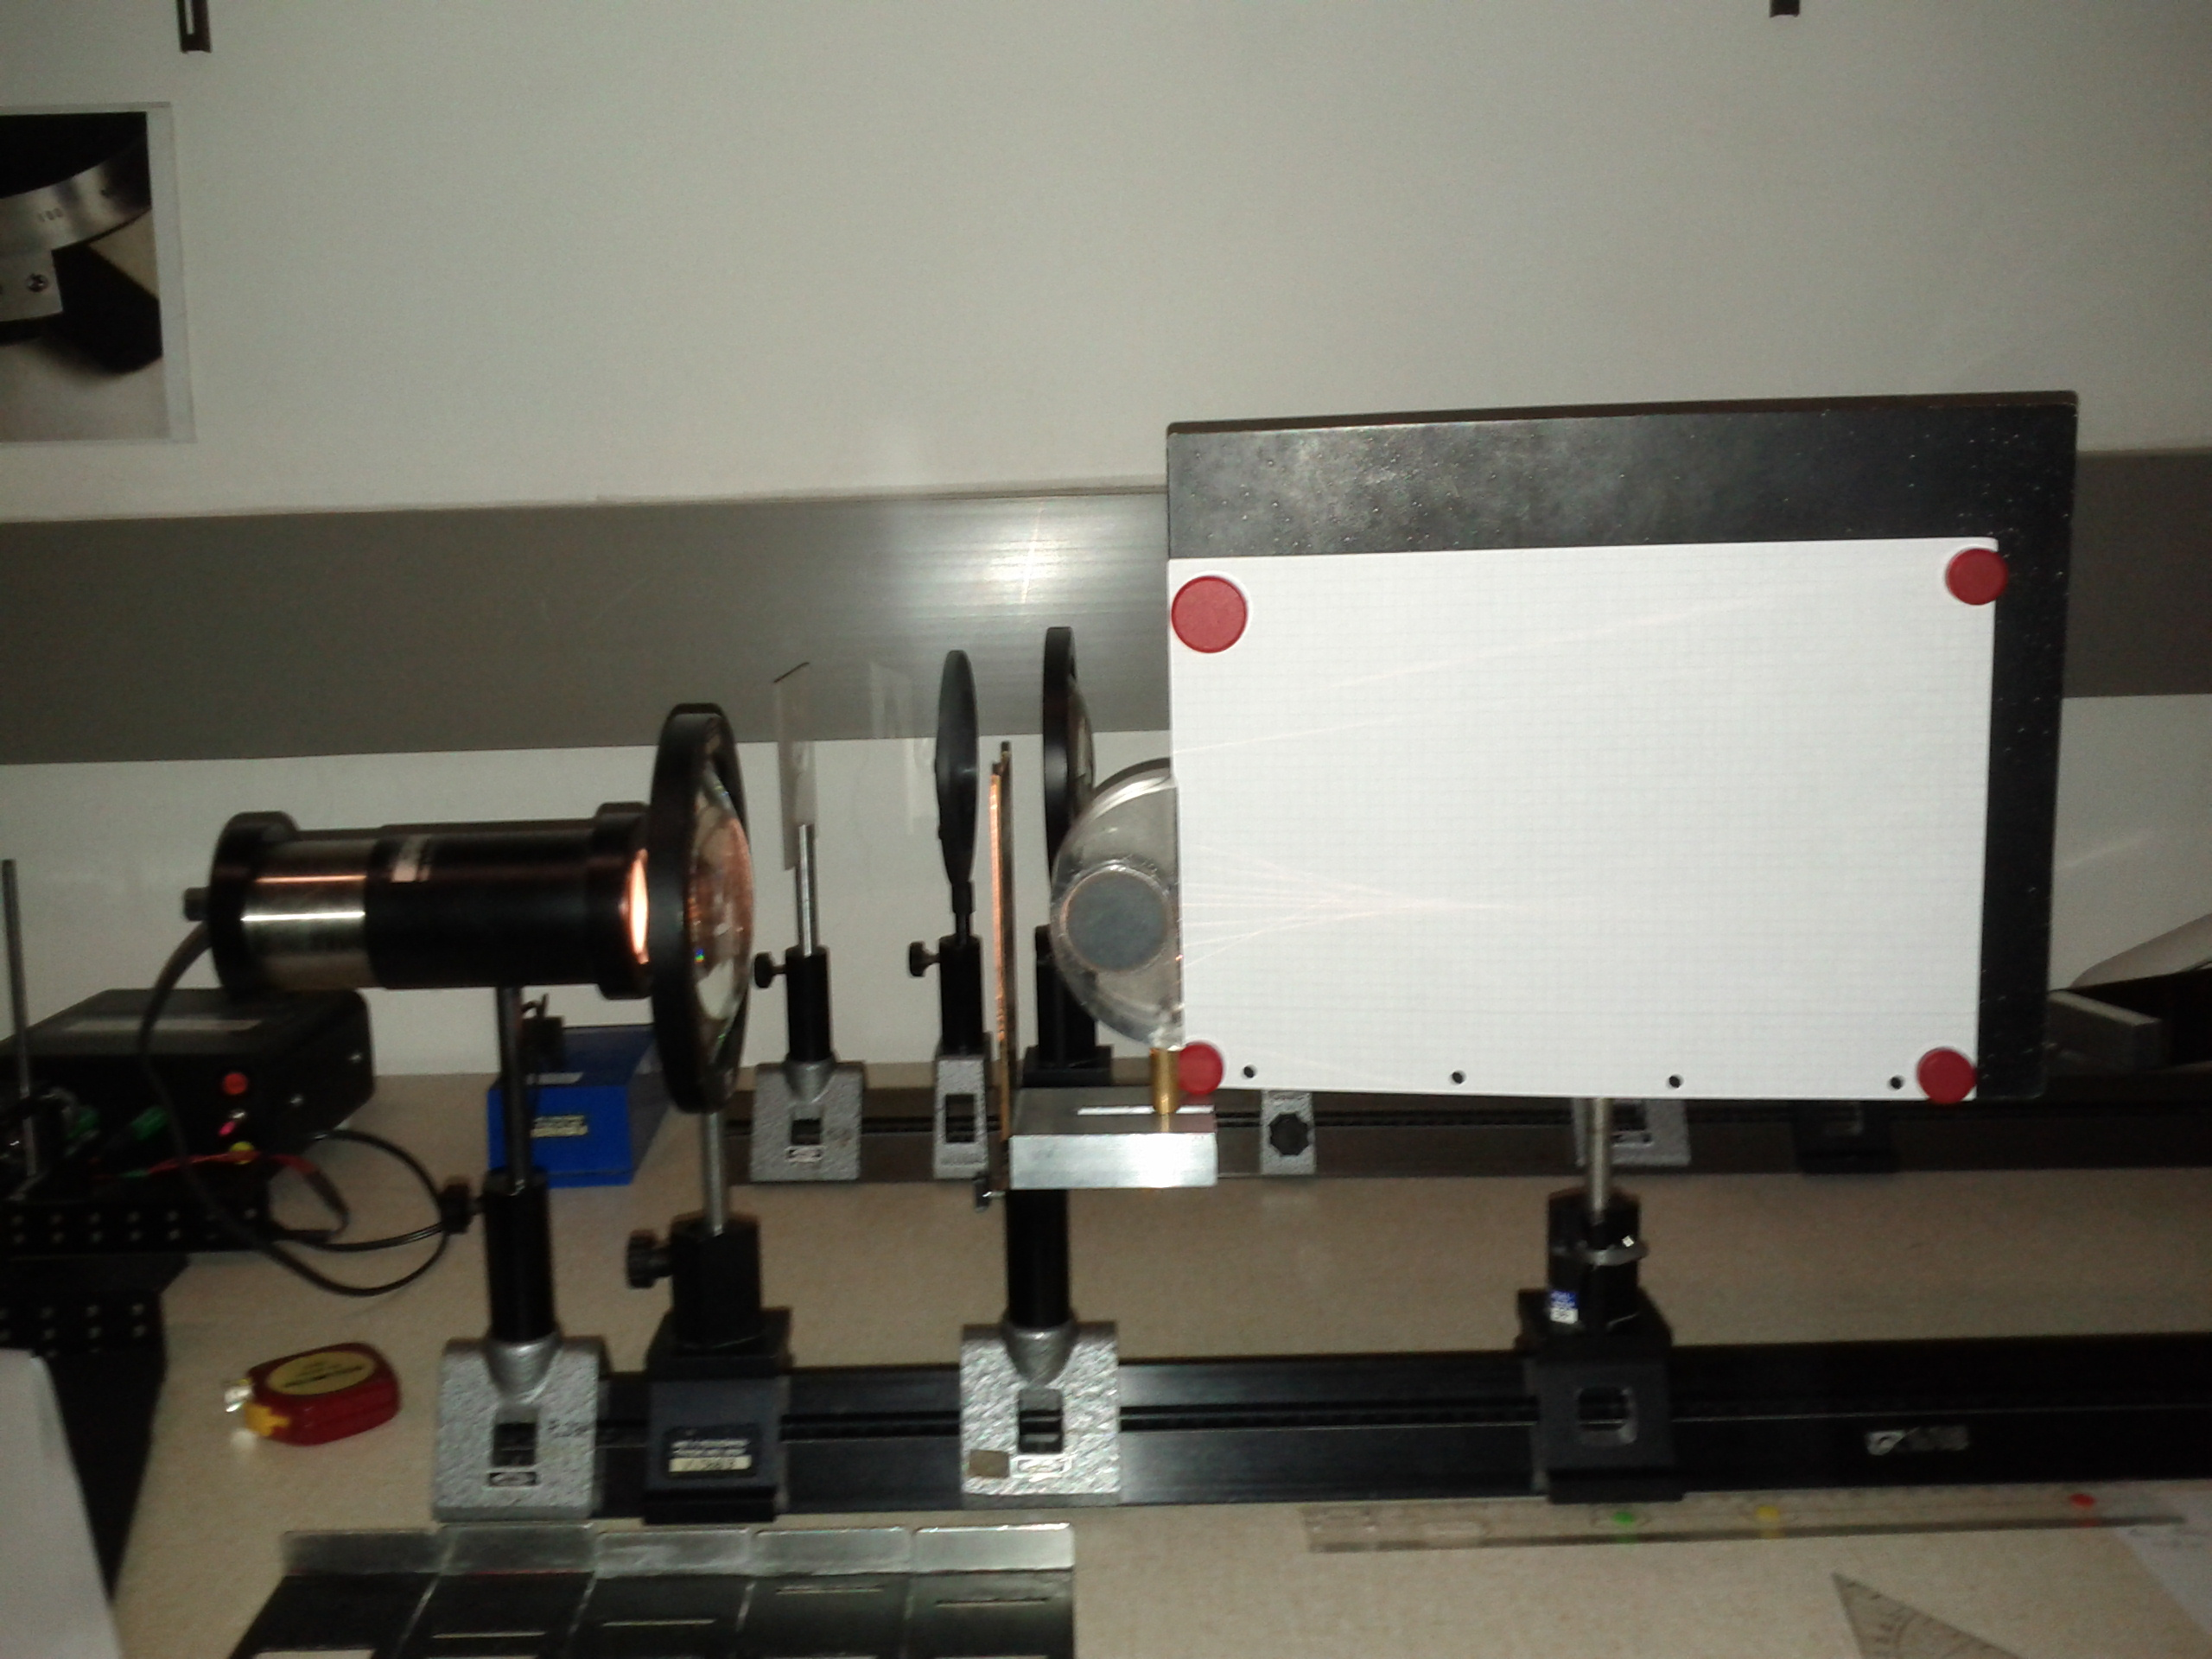
\includegraphics[scale=0.13]{./figure/linsenfehler.jpg}
%	\caption{Versuchaufbau Konvex-Plan Linse}
%	\label{fig:linsenfehler_aufbau}
%\end{figure}

%%%%%%%%%%%%%%%%%%%%%%%%%%%%%%%%%%%%%%%%%%%%%%%%
\section{Dispersionskurve eines Glasprismas}
Cadmiumlampe, 5 Linien, 

\subsection{Messwerte und Ergebnisse}

\begin{figure}[H]
	\centering
	\pgfplotstabletypeset[
			columns={w,lambda},
			col sep=&,
			columns/w/.style={string type, column name=\makecell{$Winkel$\\$[Grad]$} }, 
			columns/lambda/.style={column name=\makecell{$Wellenlänge$\\$[nm]$}, precision=0},
			every head row/.style={before row=\hline,after row=\hline\hline},
			every last row/.style={after row=\hline},
			every first column/.style={column type/.add={|}{} },
			every last column/.style={column type/.add={}{|} }
			]{
			w & lambda
			$47^\circ 50'$ & 550
			
			}
	\caption{Messwerte Winkel und Wellenlänge Cadmium Dampflampe}
	\label{fig:werte_cadmiumdampflampe}
\end{figure}

\subsection{Diskussion}


%%%%%%%%%%%%%%%%%%%%%%%%%%%%%%%%%%%%%%%%%%%%%%%%
\section{Lichtbrechung an einer planparallelen Platte}

\subsection{Messwerte und Ergebnisse}


\subsection{Diskussion}


%%%%%%%%%%%%%%%%%%%%%%%%%%%%%%%%%%%%%%%%%%%%%%%%
\section{Refraktometrie}

\subsection{Messwerte und Ergebnisse}


\subsection{Diskussion}


\section{Quellen}
$[1]$ Leitfaden, \url{http://www.univie.ac.at/anfpra/neu1/pw/pw6/PW6PL4.pdf}\\

\end{multicols}
\end{document}